\documentclass[11pt,letterpaper]{article}
\usepackage[utf8]{inputenc}
\usepackage[T1]{fontenc}
\usepackage[english]{babel}
\usepackage{lmodern}
\usepackage{amsmath,amssymb,amsfonts}
\usepackage[margin=2.5cm]{geometry}
\usepackage{fancyhdr}
\usepackage{enumitem}
\usepackage[most]{tcolorbox}
\usepackage{xcolor}
\usepackage{colortbl}
\usepackage{tikz}
\usetikzlibrary{arrows.meta,angles,quotes,calc,babel,decorations.markings}
\usepackage{placeins}
\usepackage{needspace}

% ============ PALETTE: BLACK, ORANGE, AND CREAM ============
\definecolor{blackmain}{HTML}{1A1A1A}
\definecolor{orangeacc}{HTML}{E65C00}
\definecolor{creambg}{HTML}{FBF8F1}
\definecolor{orangebg}{HTML}{FFF4EB}
\definecolor{graymuted}{HTML}{7A746E}
\definecolor{pureblack}{HTML}{0D0D0D}

% ============ HEADERS AND FOOTERS ============
\setlength{\headheight}{24pt}
\pagestyle{fancy}
\fancyhf{}
\fancyhead[L]{\textcolor{blackmain}{\textbf{\small Mathematical Methods I}}}
\fancyhead[R]{\textcolor{orangeacc}{\textbf{\small Circulation and Differential Forms}}}
\fancyfoot[C]{\textcolor{graymuted}{\thepage}}
\renewcommand{\headrulewidth}{0.8pt}
\renewcommand{\headrule}{\hbox to\headwidth{\color{orangeacc}\leaders\hrule height \headrulewidth\hfill}}

\setlist[itemize]{label={\small\textcolor{orangeacc}{$\blacksquare$}},leftmargin=1.6em}
\setlist[enumerate]{label={\textcolor{orangeacc}{\arabic*.}},leftmargin=1.8em}

% ============ TITLES ============
\newcommand{\manualsection}[1]{%
  \Needspace{12\baselineskip}%
  \vspace{0.35cm}
  \par\noindent{\Large\bfseries\color{blackmain} #1}\par\nobreak
  \noindent{\color{orangeacc}\rule{\linewidth}{1.4pt}}\par\nobreak
  \vspace{0.15cm}
}

\newcommand{\manualsubsection}[1]{%
  \Needspace{5\baselineskip}%
  \par\vspace{0.2cm}\noindent{\bfseries\color{orangeacc} #1}\par\nobreak
  \vspace{0.12cm}
}

% ============ CONTENT BOXES ============
\newtcolorbox{infobox}[2][orangeacc]{
  enhanced,
  colback=creambg,colframe=#1!90!black,
  boxrule=1pt,arc=2mm,
  left=9pt,right=9pt,top=8pt,bottom=8pt,
  before upper={\textbf{\color{#1!95!black}\large #2}\par\nobreak
    {\color{#1!50}\rule{\linewidth}{0.6pt}}\par\nobreak\smallskip}
}

\newtcolorbox{examplebox}[1]{
  enhanced,
  colback=orangebg,colframe=orangeacc!85!black,
  boxrule=1pt,arc=2mm,
  left=9pt,right=9pt,top=8pt,bottom=8pt,
  before upper={\textbf{\color{orangeacc!95!black}\large #1}\par\nobreak
    {\color{orangeacc!40}\rule{\linewidth}{0.6pt}}\par\nobreak\smallskip}
}

\newtcolorbox{theorembox}[1]{
  enhanced,
  colback=creambg!70!white,colframe=pureblack,
  boxrule=1.1pt,arc=2mm,
  left=9pt,right=9pt,top=8pt,bottom=8pt,
  before upper={\textbf{\color{pureblack}\large #1}\par\nobreak
    {\color{orangeacc}\rule{\linewidth}{0.8pt}}\par\nobreak\smallskip}
}

\newcommand{\term}[1]{\textbf{\color{orangeacc}#1}}
\newcommand{\termb}[1]{\textbf{\color{blackmain}#1}}
\renewcommand{\familydefault}{\rmdefault}
\tikzset{every node/.append style={font=\rmfamily}}
\tikzset{midarrow/.style={postaction={decorate},decoration={markings,
  mark=at position 0.5 with {\arrow{Stealth[length=5pt]}}}}}

\begin{document}
\color{blackmain}

\begin{center}
  {\LARGE\textbf{\color{blackmain}Mathematical Methods I}}\\[0.2cm]
  {\Large\textcolor{orangeacc}{\textbf{Circulation, Density, and Orientation}}}\\[0.4cm]
  {\large\textcolor{graymuted}{Gabriel Velázquez}}\\[0.35cm]
\end{center}

% =====================================================================
\manualsection{1. Circulation Along a Loop}

Let $\mathbf{V}$ be a vector field: the velocity of a fluid or a force.
We walk along a closed curve $C$ and, at each point, ask whether the field
\emph{pushes along} or \emph{against} the direction in which we are walking.
Only the component of $\mathbf{V}$ \emph{tangent} to the curve matters; the
perpendicular component does not contribute to the trip.

\begin{infobox}[orangeacc]{Definition 1.1 (Circulation)}
Let $C$ be an oriented closed curve, parametrized by
$\mathbf{r}(t)=(x(t),y(t),z(t))$ with $a\le t\le b$, and let
$\mathbf{V}=(P,Q,R)$ be a continuous field. The \term{circulation} of
$\mathbf{V}$ along $C$ is
\begin{equation}
  \oint_C \mathbf{V}\cdot d\mathbf{r}
  =\oint_C V_T\,ds
  =\int_a^b \mathbf{V}(\mathbf{r}(t))\cdot\mathbf{r}'(t)\,dt,
  \qquad V_T=\mathbf{V}\cdot\mathbf{T},
\end{equation}
where $\mathbf{T}$ is the unit tangent vector. With the 1-form
$\alpha=P\,dx+Q\,dy+R\,dz$ associated with the field, this is written
\begin{equation}
  \oint_C\alpha=\int_a^b\bigl(P\,x'+Q\,y'+R\,z'\bigr)\,dt .
\end{equation}
\end{infobox}

The 1-form $\alpha$ acts as a machine that \emph{consumes} the velocity vector
$\mathbf{r}'(t)$ of the trip and returns a number:
$\alpha_p(\mathbf{w})=\mathbf{V}(p)\cdot\mathbf{w}$. The integral adds up those
numbers along the curve. Note that the integral only needs $\alpha$ and the
curve; it does not require a metric to measure lengths.

\begin{figure}[htbp]
\centering
\begin{tikzpicture}[scale=1.15,>=Stealth]
  \draw[graymuted,thick] (0,0) ellipse (2.6 and 1.7);
  \draw[->,graymuted!70!black,very thick] (1.84,1.2)--++(-0.35,0.23);
  \node[graymuted] at (-1.6,-1.7) {$C$};
  % right point: along the curve
  \fill[blackmain] (2.6,0) circle (2pt);
  \draw[->,orangeacc,very thick] (2.6,0)--(3.1,1.2) node[right] {$\mathbf{V}$};
  \draw[->,blackmain,very thick] (2.6,0)--(2.6,1.2);
  \node[blackmain,anchor=north west] at (2.68,-0.05) {\small $V_T>0$};
  % top point: perpendicular
  \fill[blackmain] (0,1.7) circle (2pt);
  \draw[->,orangeacc,very thick] (0,1.7)--(0,2.7) node[above] {$\mathbf{V}$};
  \node[blackmain,below] at (0,1.55) {\small $V_T=0$};
  % left point: against the curve
  \fill[blackmain] (-2.6,0) circle (2pt);
  \draw[->,orangeacc,very thick] (-2.6,0)--(-2.9,1.1) node[left] {$\mathbf{V}$};
  \draw[->,blackmain,very thick] (-2.6,0)--(-2.6,1.1);
  \node[blackmain,left] at (-2.6,-0.5) {\small $V_T<0$};
  % bottom point: along the curve
  \fill[blackmain] (0,-1.7) circle (2pt);
  \draw[->,orangeacc,very thick] (0,-1.7)--(1.3,-1.45) node[right] {$\mathbf{V}$};
  \draw[->,blackmain,very thick] (0,-1.7)--(1.3,-1.7);
  \node[blackmain,below] at (0.7,-1.75) {\small $V_T>0$};
\end{tikzpicture}
\caption{The curve is traversed counterclockwise. The orange arrows are the
field $\mathbf{V}$; the black ones are its projection $V_T$ onto the direction
of travel. Where the field helps the trip it contributes a $+$ sign; where it
opposes the trip, a $-$ sign; where it is perpendicular, it contributes
nothing.}
\label{fig:circulacion}
\end{figure}
\FloatBarrier

\begin{infobox}[blackmain]{Two Physical Readings of the Same Integral}
\begin{itemize}
  \item \termb{Fluids:} if $\mathbf{V}$ is the velocity, the circulation
        measures the overall tendency of the fluid to rotate around $C$. A
        paddle wheel placed in the flow turns when the velocity is greater on
        one side than on the other.
  \item \termb{Forces:} if $\mathbf{V}=\mathbf{F}$ is a force field, the
        circulation is the total work done in carrying a particle around the
        closed path.
\end{itemize}
Reversing the orientation changes the sign: $\oint_{-C}\alpha=-\oint_C\alpha$.
\end{infobox}

\begin{examplebox}{Example 1.2 (Two Fields on the Unit Circle)}
Let $C$: $\mathbf{r}(t)=(\cos t,\sin t)$, $0\le t\le2\pi$, with
$\mathbf{r}'(t)=(-\sin t,\cos t)$.
\begin{itemize}
  \item \termb{Rotation field} $\mathbf{V}=(-y,x)$, that is,
        $\alpha=-y\,dx+x\,dy$. Here $\mathbf{V}(\mathbf{r}(t))=(-\sin t,\cos t)$
        coincides with $\mathbf{r}'(t)$, so
        \[
          \oint_C\alpha=\int_0^{2\pi}(\sin^2t+\cos^2t)\,dt=2\pi .
        \]
        Traversed backwards, the circulation is $-2\pi$.
  \item \termb{Radial field} $\mathbf{V}=(x,y)$, that is, $\alpha=x\,dx+y\,dy$.
        Now $\mathbf{V}\cdot\mathbf{r}'=-\cos t\sin t+\sin t\cos t=0$ at every
        point: the field is perpendicular to the curve and the circulation is
        $0$.
\end{itemize}
\end{examplebox}

% =====================================================================
\manualsection{2. How to Compute It: the Square}

For a curve with corners, the boundary is divided into smooth pieces and the
integrals over each piece are added. Consider the square
$Q=[0,a]\times[0,a]$ traversed counterclockwise and the 1-form
$\alpha=P(x,y)\,dx+Q(x,y)\,dy$.

\begin{theorembox}{Proposition 2.1 (Circulation Around a Square)}
The boundary $\partial Q$ consists of four pieces:
\begin{center}
\renewcommand{\arraystretch}{2.1}
\begin{tabular}{llll}
  $C_1$ (bottom): & $y=0,\ dy=0$ & $x:0\to a$ & $\displaystyle\int_0^a P(x,0)\,dx$\\
  $C_2$ (right): & $x=a,\ dx=0$ & $y:0\to a$ & $\displaystyle\int_0^a Q(a,y)\,dy$\\
  $C_3$ (top): & $y=a,\ dy=0$ & $x:a\to0$ & $\displaystyle-\int_0^a P(x,a)\,dx$\\
  $C_4$ (left): & $x=0,\ dx=0$ & $y:a\to0$ & $\displaystyle-\int_0^a Q(0,y)\,dy$
\end{tabular}
\end{center}
and therefore
\begin{equation}
  \oint_{\partial Q}\alpha
  =\int_0^a\bigl[P(x,0)-P(x,a)\bigr]\,dx
  +\int_0^a\bigl[Q(a,y)-Q(0,y)\bigr]\,dy .
\end{equation}
\end{theorembox}

The negative sign on $C_3$ and $C_4$ appears because they are traversed against
the direction of the axes. This is why opposite sides are \emph{subtracted}:
what matters is how much $P$ changes from bottom to top and how much $Q$ changes
from left to right. This observation is the seed of the circulation density in
the next section.

\begin{figure}[htbp]
\centering
\begin{tikzpicture}[scale=2.0,>=Stealth]
  \draw[->,graymuted] (-0.3,0)--(2.7,0) node[right] {$x$};
  \draw[->,graymuted] (0,-0.3)--(0,2.7) node[above] {$y$};
  \fill[orangebg] (0,0) rectangle (2,2);
  \foreach \xx in {0,1,2} {
    \foreach \yy in {0,1,2} {
      \pgfmathtruncatemacro{\nz}{abs(\xx)+abs(\yy)}\ifnum\nz>0
        \draw[->,graymuted!70] (\xx,\yy)--++({-0.25*\yy},{0.25*\xx});
      \fi
    }
  }
  \draw[orangeacc,very thick,midarrow] (0,0)--(2,0);
  \draw[orangeacc,very thick,midarrow] (2,0)--(2,2);
  \draw[orangeacc,very thick,midarrow] (2,2)--(0,2);
  \draw[orangeacc,very thick,midarrow] (0,2)--(0,0);
  \node[blackmain,below] at (1,-0.04) {\small $C_1$: contributes $0$};
  \node[blackmain,right] at (2.04,1) {\small $C_2$: $4$};
  \node[blackmain,above] at (1,2.04) {\small $C_3$: $4$};
  \node[blackmain,left] at (-0.04,1) {\small $C_4$: $0$};
  \node[blackmain,fill=orangebg,inner sep=3pt] at (1.0,1.0) {\large $\oint_{\partial Q}\alpha=8$};
\end{tikzpicture}
\caption{Square $[0,2]^2$ with the field $(-y,x)$ from Example 2.2 (gray
arrows, drawn at reduced scale). The bottom and left sides are
\emph{perpendicular} to the field and contribute nothing; the right and top
sides go along the field and contribute $4$ each.}
\label{fig:cuadrado}
\end{figure}
\FloatBarrier

\begin{examplebox}{Example 2.2 (Circulation of $-y\,dx+x\,dy$ on $[0,2]^2$)}
With $a=2$:
\begin{itemize}
  \item $C_1$: $y=0$, so $\alpha=0$ and the integral is $0$.
  \item $C_2$: $x=2$, $dx=0$: $\displaystyle\int_0^2 2\,dy=4$.
  \item $C_3$: $y=2$, $dy=0$, $x$ from $2$ to $0$:
        $\displaystyle\int_2^0(-2)\,dx=4$.
  \item $C_4$: $x=0$, so $\alpha=0$ and the integral is $0$.
\end{itemize}
Total: $\oint_{\partial Q}\alpha=0+4+4+0=\mathbf{8}$. Since the area of the
square is $4$, the result is exactly $2\times\text{area}$. This is no
coincidence; it is explained in Section 3.
\end{examplebox}

% =====================================================================
\manualsection{3. Shrinking the Loop: Circulation Density}

The circulation depends on the chosen loop. To know what the field does \emph{at
a point}, we shrink the loop around it and normalize by the enclosed area.

\begin{infobox}[orangeacc]{Definition 3.1 (Circulation Density)}
Let $p$ be a point, and let $\partial(\Delta A)$ be the counterclockwise
boundary of a small region of area $\Delta A$ containing $p$. The
\term{circulation density} of $\alpha$ at $p$ is
\begin{equation}
  \lim_{\Delta A\to0}\frac{1}{\Delta A}\oint_{\partial(\Delta A)}\alpha .
\end{equation}
It is the local rate of rotation of the field: the circulation \emph{per unit
area}.
\end{infobox}

To compute it we take an infinitesimal rectangle
$[x,x+\Delta x]\times[y,y+\Delta y]$ and approximate each side by the value of
the integrand at its starting point.

\begin{figure}[htbp]
\centering
\begin{tikzpicture}[scale=1.0,>=Stealth]
  \fill[orangebg] (0,0) rectangle (6,3.4);
  \draw[orangeacc,very thick,midarrow] (0,0)--(6,0);
  \draw[orangeacc,very thick,midarrow] (6,0)--(6,3.4);
  \draw[orangeacc,very thick,midarrow] (6,3.4)--(0,3.4);
  \draw[orangeacc,very thick,midarrow] (0,3.4)--(0,0);
  \fill[blackmain] (0,0) circle (2pt) node[below left] {$(x,y)$};
  \fill[blackmain] (6,0) circle (2pt) node[below right] {$(x+\Delta x,\,y)$};
  \fill[blackmain] (6,3.4) circle (2pt) node[above right] {$(x+\Delta x,\,y+\Delta y)$};
  \fill[blackmain] (0,3.4) circle (2pt) node[above left] {$(x,\,y+\Delta y)$};
  \node[blackmain,above] at (3,0.05) {\small $P(x,y)\,\Delta x$};
  \node[blackmain,below] at (3,3.35) {\small $-P(x,y+\Delta y)\,\Delta x$};
  \node[blackmain,rotate=90,above] at (6.0,1.7) {\small $Q(x+\Delta x,y)\,\Delta y$};
  \node[blackmain,rotate=90,below] at (0.0,1.7) {\small $-Q(x,y)\,\Delta y$};
  \node[blackmain] at (3,1.7) {\small $\displaystyle\oint\approx
    \Bigl(\frac{\partial Q}{\partial x}-\frac{\partial P}{\partial y}\Bigr)\Delta x\,\Delta y$};
\end{tikzpicture}
\caption{Contribution of each side of the infinitesimal rectangle. On the top
and bottom, the values of $P$ at two heights are compared; on the left and
right, the values of $Q$ at two positions.}
\label{fig:rectangulo}
\end{figure}
\FloatBarrier

Adding the four sides:
\begin{align*}
  \oint_{\partial(\Delta A)}\alpha
  &\approx P(x,y)\Delta x+Q(x+\Delta x,y)\Delta y
          -P(x,y+\Delta y)\Delta x-Q(x,y)\Delta y\\
  &=-\bigl[P(x,y+\Delta y)-P(x,y)\bigr]\Delta x
    +\bigl[Q(x+\Delta x,y)-Q(x,y)\bigr]\Delta y\\
  &\approx\Bigl(\frac{\partial Q}{\partial x}-\frac{\partial P}{\partial y}\Bigr)
    \Delta x\,\Delta y .
\end{align*}

\begin{theorembox}{Theorem 3.2 (Circulation Density in the Plane)}
If $\alpha=P\,dx+Q\,dy$ is of class $C^1$, its circulation density at
$(x,y)$ is
\begin{equation}
  \frac{\partial Q}{\partial x}-\frac{\partial P}{\partial y}.
\end{equation}
\end{theorembox}

\manualsubsection{How to Read the Sign}
\begin{itemize}
  \item $\partial Q/\partial x>0$: the vertical component of the field grows
        toward the right. The right side (which we traverse upward) receives
        more push than the left side (which we traverse downward):
        counterclockwise rotation, contribution $+$.
  \item $\partial P/\partial y>0$: the horizontal component grows upward. On
        the top side we move to the left, against the push, which is stronger
        there than at the bottom: clockwise rotation, contribution $-$.
\end{itemize}

\begin{figure}[htbp]
\centering
\begin{tikzpicture}[scale=1.0,>=Stealth]
  % Panel 1: rigid rotation
  \begin{scope}
    \node[blackmain] at (0,2.95) {\small $\mathbf{V}=(-y,x)$};
    \foreach \xx in {-2,-1,0,1,2} {
      \foreach \yy in {-2,-1,0,1,2} {
        \fill[graymuted] (\xx,\yy) circle (0.8pt);
        \pgfmathtruncatemacro{\nz}{abs(\xx)+abs(\yy)}\ifnum\nz>0
          \draw[->,orangeacc,thick] (\xx,\yy)--++({-0.28*\yy},{0.28*\xx});
        \fi
      }
    }
    \draw[->,blackmain,very thick] ([shift={(40:0.4)}]0.0,0.0) arc (40:330:0.4);
    \node[blackmain,align=center] at (0,-3.15) {\small density $=2$\\[-1pt]\small (counterclockwise)};
  \end{scope}
  % Panel 2: shear
  \begin{scope}[xshift=5.5cm]
    \node[blackmain] at (0,2.95) {\small $\mathbf{V}=(y,0)$};
    \foreach \xx in {-2,-1,0,1,2} {
      \foreach \yy in {-2,-1,0,1,2} {
        \fill[graymuted] (\xx,\yy) circle (0.8pt);
        \ifnum\yy=0
        \else
          \draw[->,orangeacc,thick] (\xx,\yy)--++({0.28*\yy},0);
        \fi
      }
    }
    \draw[->,blackmain,very thick] ([shift={(140:0.4)}]0.0,0.0) arc (140:-150:0.4);
    \node[blackmain,align=center] at (0,-3.15) {\small density $=-1$\\[-1pt]\small (clockwise)};
  \end{scope}
  % Panel 3: radial
  \begin{scope}[xshift=11cm]
    \node[blackmain] at (0,2.95) {\small $\mathbf{V}=(x,y)$};
    \foreach \xx in {-2,-1,0,1,2} {
      \foreach \yy in {-2,-1,0,1,2} {
        \fill[graymuted] (\xx,\yy) circle (0.8pt);
        \pgfmathtruncatemacro{\nz}{abs(\xx)+abs(\yy)}\ifnum\nz>0
          \draw[->,orangeacc,thick] (\xx,\yy)--++({0.28*\xx},{0.28*\yy});
        \fi
      }
    }
    \node[blackmain,align=center] at (0,-3.15) {\small density $=0$\\[-1pt]\small (no rotation)};
  \end{scope}
\end{tikzpicture}
\caption{Three fields with constant circulation density. A paddle wheel placed
at any point turns counterclockwise in the first, turns clockwise in the
second, and does not turn in the third.}
\label{fig:tres-campos}
\end{figure}
\FloatBarrier

\begin{examplebox}{Example 3.3 (Three Fields, Three Behaviors)}
\begin{itemize}
  \item $\alpha=-y\,dx+x\,dy$: $\ \partial_xQ-\partial_yP=1-(-1)=2$. This is a
        rigid rotation with angular velocity $1$. It explains the result of
        Example 2.2: circulation $=2\times\text{area}=2\times4=8$.
        In general, the circulation density of a fluid is twice its local
        angular velocity.
  \item $\alpha=y\,dx$: $\ \partial_xQ-\partial_yP=0-1=-1$. \emph{The
        streamlines are straight}, and yet there is rotation: the paddle wheel
        turns because the velocity changes from one layer to the next.
  \item $\alpha=x\,dx+y\,dy$: $\ \partial_xQ-\partial_yP=0-0=0$. A radial field
        expands the fluid but does not make it rotate.
\end{itemize}
\end{examplebox}

% =====================================================================
\manualsection{4. Oriented Area and the Wedge Product}

The circulation depends on the direction of travel (counterclockwise or
clockwise). To rebuild it as \emph{density $\times$ area} we need a notion of
area that also carries a direction: a signed area. That is a 2-form.

\begin{infobox}[orangeacc]{Definition 4.1 (The 2-Form $dx\wedge dy$)}
$dx\wedge dy$ is a function that takes \emph{two} vectors
$\mathbf{u}=(u_1,u_2)$ and $\mathbf{v}=(v_1,v_2)$ and returns the oriented area
of the parallelogram they span:
\begin{equation}
  (dx\wedge dy)(\mathbf{u},\mathbf{v})
  =u_1v_2-u_2v_1
  =\det\begin{pmatrix}u_1&v_1\\u_2&v_2\end{pmatrix}.
\end{equation}
The sign is $+$ if going from $\mathbf{u}$ to $\mathbf{v}$ through the smaller
angle is counterclockwise, and $-$ if it is clockwise.
\end{infobox}

\begin{figure}[htbp]
\centering
\begin{tikzpicture}[scale=1.25,>=Stealth]
  \begin{scope}
    \fill[orangebg] (0,0)--(2,0)--(3,1)--(1,1)--cycle;
    \draw[graymuted,dashed] (2,0)--(3,1)--(1,1);
    \draw[->,orangeacc,very thick] (0,0)--(2,0) node[midway,below] {$\mathbf{u}$ (1st)};
    \draw[->,blackmain,very thick] (0,0)--(1,1) node[midway,above left] {$\mathbf{v}$ (2nd)};
    \draw[->,orangeacc,thick] ([shift={(30:0.32)}]1.5,0.5) arc (30:330:0.32);
    \node[blackmain,align=center] at (1.5,-1.0)
      {\small $(dx\wedge dy)(\mathbf{u},\mathbf{v})=+2$\\[-1pt]\small counterclockwise};
  \end{scope}
  \begin{scope}[xshift=6.2cm]
    \fill[orangebg] (0,0)--(1,1)--(3,1)--(2,0)--cycle;
    \draw[graymuted,dashed] (1,1)--(3,1)--(2,0);
    \draw[->,orangeacc,very thick] (0,0)--(1,1) node[midway,above left] {$\mathbf{v}$ (1st)};
    \draw[->,blackmain,very thick] (0,0)--(2,0) node[midway,below] {$\mathbf{u}$ (2nd)};
    \draw[->,orangeacc,thick] ([shift={(30:0.32)}]1.5,0.5) arc (30:-270:0.32);
    \node[blackmain,align=center] at (1.5,-1.0)
      {\small $(dx\wedge dy)(\mathbf{v},\mathbf{u})=-2$\\[-1pt]\small clockwise};
  \end{scope}
\end{tikzpicture}
\caption{With $\mathbf{u}=(2,0)$ and $\mathbf{v}=(1,1)$ the parallelogram has
area $2$ in both cases. What changes is the \emph{order} of the vectors and,
with it, the direction in which the boundary is traversed. Swapping the order
flips the sign.}
\label{fig:area-orientada}
\end{figure}
\FloatBarrier

\begin{theorembox}{Proposition 4.2 (Properties of the Wedge Product)}
For 1-forms $\omega,\eta$ and scalars $a,b$:
\begin{equation}
  dx\wedge dy=-\,dy\wedge dx,\qquad
  dx\wedge dx=0,\qquad
  \omega\wedge(a\eta)=a\,(\omega\wedge\eta).
\end{equation}
The second identity says that two parallel vectors span a degenerate
parallelogram, of area $0$.
\end{theorembox}

\manualsubsection{In $\mathbb{R}^3$: Three Planes, Three Areas}
A parallelogram in space has three \emph{shadows} on the coordinate planes,
and each shadow is an oriented area:
\begin{equation}
  (dy\wedge dz)(\mathbf{u},\mathbf{v})=u_2v_3-u_3v_2,\quad
  (dz\wedge dx)(\mathbf{u},\mathbf{v})=u_3v_1-u_1v_3,\quad
  (dx\wedge dy)(\mathbf{u},\mathbf{v})=u_1v_2-u_2v_1 .
\end{equation}
These three quantities are exactly the components of the cross product
$\mathbf{u}\times\mathbf{v}$: the normal vector whose length is the area and
whose direction gives the orientation.

\begin{figure}[htbp]
\centering
\begin{tikzpicture}[x={(-0.6cm,-0.5cm)},y={(1cm,0cm)},z={(0cm,1cm)},scale=1.5,>=Stealth]
  \draw[->,graymuted] (0,0,0)--(2.9,0,0) node[below left] {$x$};
  \draw[->,graymuted] (0,0,0)--(0,3.5,0) node[right] {$y$};
  \draw[->,graymuted] (0,0,0)--(0,0,2.4) node[above] {$z$};
  % shadow
  \fill[orangeacc!25] (0.2,0.3,0)--(1.7,0.3,0)--(2.1,2.7,0)--(0.6,2.7,0)--cycle;
  \draw[orangeacc,dashed] (0.2,0.3,0)--(1.7,0.3,0)--(2.1,2.7,0)--(0.6,2.7,0)--cycle;
  % vertical projections
  \draw[graymuted,dotted] (0.2,0.3,0)--(0.2,0.3,0.4);
  \draw[graymuted,dotted] (1.7,0.3,0)--(1.7,0.3,1.6);
  \draw[graymuted,dotted] (2.1,2.7,0)--(2.1,2.7,1.6);
  \draw[graymuted,dotted] (0.6,2.7,0)--(0.6,2.7,0.4);
  % parallelogram
  \fill[blackmain!10,opacity=0.85] (0.2,0.3,0.4)--(1.7,0.3,1.6)--(2.1,2.7,1.6)--(0.6,2.7,0.4)--cycle;
  \draw[blackmain,thick] (0.2,0.3,0.4)--(1.7,0.3,1.6)--(2.1,2.7,1.6)--(0.6,2.7,0.4)--cycle;
  \draw[->,orangeacc,very thick] (0.2,0.3,0.4)--(1.7,0.3,1.6) node[midway,above=4pt] {$\mathbf{u}$};
  \draw[->,blackmain,very thick] (0.2,0.3,0.4)--(0.6,2.7,0.4) node[midway,below] {$\mathbf{v}$};
  \node[orangeacc,align=left,anchor=west] at (1.0,3.6,0)
    {\small shadow on the $xy$ plane:\\[-1pt]\small $(dx\wedge dy)(\mathbf{u},\mathbf{v})$};
\end{tikzpicture}
\caption{A parallelogram in $\mathbb{R}^3$ and its shadow on the $xy$ plane
(orange). Evaluating $dx\wedge dy$ at $(\mathbf{u},\mathbf{v})$ measures the
oriented area of the shadow. Likewise, $dy\wedge dz$ and $dz\wedge dx$ measure
the shadows on the other two planes.}
\label{fig:sombra}
\end{figure}
\FloatBarrier

\begin{examplebox}{Example 4.3 (The Three Shadows)}
Let $\mathbf{u}=(1.5,\,0,\,1.2)$ and $\mathbf{v}=(0.4,\,2.4,\,0)$ be the vectors
in Figure~\ref{fig:sombra}. Then
\begin{align*}
  (dy\wedge dz)(\mathbf{u},\mathbf{v})&=0(0)-1.2(2.4)=-2.88,\\
  (dz\wedge dx)(\mathbf{u},\mathbf{v})&=1.2(0.4)-1.5(0)=0.48,\\
  (dx\wedge dy)(\mathbf{u},\mathbf{v})&=1.5(2.4)-0(0.4)=3.6,
\end{align*}
and indeed $\mathbf{u}\times\mathbf{v}=(-2.88,\,0.48,\,3.6)$. The shadow on the
$xy$ plane is the largest, and the one on the $zx$ plane is very small: the
normal vector points mostly along $z$, and the negative sign of the first
component indicates that the shadow on the $yz$ plane is oppositely oriented.
\end{examplebox}

% =====================================================================
\manualsection{5. The Exterior Derivative: Density $\times$ Oriented Area}

We now have the two ingredients: the circulation density (Section 3) and the
oriented area (Section 4). The exterior derivative $d$ combines them into a
single object.

\begin{infobox}[orangeacc]{Definition 5.1 (Exterior Derivative of a 1-Form)}
For $\alpha=P\,dx+Q\,dy+R\,dz$ the 2-form $d\alpha$ is defined by
\begin{equation}
  d\alpha
  =\Bigl(\frac{\partial R}{\partial y}-\frac{\partial Q}{\partial z}\Bigr)dy\wedge dz
  +\Bigl(\frac{\partial P}{\partial z}-\frac{\partial R}{\partial x}\Bigr)dz\wedge dx
  +\Bigl(\frac{\partial Q}{\partial x}-\frac{\partial P}{\partial y}\Bigr)dx\wedge dy .
\end{equation}
In the plane, $d(P\,dx+Q\,dy)=\bigl(\partial_xQ-\partial_yP\bigr)\,dx\wedge dy$.
\end{infobox}

Each term has the form
\[
  \underbrace{\bigl(\text{circulation density in a coordinate plane}\bigr)}_{\text{local curl}}
  \;\times\;
  \underbrace{\bigl(\text{oriented area projected onto that plane}\bigr)}_{\text{basic 2-form}} .
\]
The three coefficients are the components of the curl
$\nabla\times\mathbf{V}$.

\begin{theorembox}{Theorem 5.2 (Geometric Meaning of $d\alpha$)}
Let $p$ be a point and $\mathbf{u},\mathbf{v}$ two vectors. If $\Pi_\varepsilon$
is the parallelogram with edges $\varepsilon\mathbf{u}$ and
$\varepsilon\mathbf{v}$ and a vertex at $p$, traversed from $\mathbf{u}$ toward
$\mathbf{v}$, then
\begin{equation}
  \oint_{\partial\Pi_\varepsilon}\alpha
  =\varepsilon^2\,(d\alpha)_p(\mathbf{u},\mathbf{v})+o(\varepsilon^2),
  \qquad
  (d\alpha)_p(\mathbf{u},\mathbf{v})=(\nabla\times\mathbf{V})(p)\cdot(\mathbf{u}\times\mathbf{v}).
\end{equation}
\end{theorembox}

In other words, \emph{the circulation around a small parallelogram is the curl
times its oriented area.} The second equality follows from comparing the
coefficients of $d\alpha$ with the components of $\mathbf{u}\times\mathbf{v}$
from Example 4.3. In the planar case with $\mathbf{u}=\Delta x\,\mathbf{e}_1$
and $\mathbf{v}=\Delta y\,\mathbf{e}_2$ it recovers the rectangle computation of
Section 3.

\begin{examplebox}{Example 5.3 (Computing $d\alpha$)}
\begin{itemize}
  \item \termb{Planar rotation.} For $\alpha=-y\,dx+x\,dy$,
        $d\alpha=\bigl(1-(-1)\bigr)dx\wedge dy=2\,dx\wedge dy$.
  \item \termb{In space.} For $\alpha=z\,dx+x\,dy+y\,dz$ we have
        $P=z$, $Q=x$, $R=y$, so
        \[
          d\alpha=(1-0)\,dy\wedge dz+(1-0)\,dz\wedge dx+(1-0)\,dx\wedge dy,
          \qquad\nabla\times\mathbf{V}=(1,1,1).
        \]
\end{itemize}
\end{examplebox}

% =====================================================================
\manualsection{6. Oriented Volume and the 3-Form $dx\wedge dy\wedge dz$}

Just as $dx\wedge dy$ measures the signed area of a parallelogram, in
$\mathbb{R}^3$ there is an analogous object for three vectors: the \emph{signed
volume} of a parallelepiped.

\begin{infobox}[orangeacc]{Definition 6.1 (Oriented Volume)}
The 3-form $dx\wedge dy\wedge dz$ takes three vectors
$\mathbf{u},\mathbf{v},\mathbf{w}\in\mathbb{R}^3$ and returns
\begin{equation}
  (dx\wedge dy\wedge dz)(\mathbf{u},\mathbf{v},\mathbf{w})
  =\det\begin{pmatrix}u_1&v_1&w_1\\u_2&v_2&w_2\\u_3&v_3&w_3\end{pmatrix}
  =\mathbf{u}\cdot(\mathbf{v}\times\mathbf{w}).
\end{equation}
Its absolute value is the volume of the parallelepiped with edges
$\mathbf{u},\mathbf{v},\mathbf{w}$. The sign is $+$ if the triple
$(\mathbf{u},\mathbf{v},\mathbf{w})$ follows the \term{right-hand rule}
(thumb, index, and middle finger), and $-$ otherwise.
\end{infobox}

The orientation of an area was read as counterclockwise or clockwise; that of a
volume is read as right-handed or left-handed. The sign rules are the same as
in Section 4:
\begin{itemize}
  \item Swapping \emph{any two} vectors flips the sign:
        $dx\wedge dy\wedge dz=-\,dy\wedge dx\wedge dz$.
  \item If the three vectors are coplanar, the parallelepiped is flat and the
        volume is $0$. In particular, any wedge product with a repeated factor
        vanishes: $dx\wedge dx\wedge dz=0$.
\end{itemize}

\begin{figure}[htbp]
\centering
\begin{tikzpicture}[x={(-0.6cm,-0.5cm)},y={(1cm,0cm)},z={(0cm,1cm)},scale=1.6,>=Stealth]
  \coordinate (O) at (0,0,0);
  \coordinate (U) at (1.5,0,0);
  \coordinate (V) at (0,2,0);
  \coordinate (W) at (0.3,0.4,1.5);
  % bottom face
  \fill[orangebg] (O)--(U)--($(U)+(V)$)--(V)--cycle;
  % top face
  \fill[orangeacc!22,opacity=0.9] (W)--($(U)+(W)$)--($(U)+(V)+(W)$)--($(V)+(W)$)--cycle;
  % front right face
  \fill[blackmain!10,opacity=0.9] (V)--($(U)+(V)$)--($(U)+(V)+(W)$)--($(V)+(W)$)--cycle;
  \draw[blackmain,thick] (O)--(U)--($(U)+(V)$)--(V)--cycle;
  \draw[blackmain,thick] (W)--($(U)+(W)$)--($(U)+(V)+(W)$)--($(V)+(W)$)--cycle;
  \draw[blackmain,thick] (O)--(W) (U)--($(U)+(W)$) (V)--($(V)+(W)$) ($(U)+(V)$)--($(U)+(V)+(W)$);
  \draw[->,orangeacc,very thick] (O)--(U) node[midway,below left] {$\mathbf{u}$};
  \draw[->,orangeacc,very thick] (O)--(V) node[midway,below] {$\mathbf{v}$};
  \draw[->,orangeacc,very thick] (O)--(W) node[midway,left] {$\mathbf{w}$};
  \fill[blackmain] (O) circle (1.6pt);
  \node[blackmain,align=center] at (0.9,1.0,-1.3)
    {\small $(dx\wedge dy\wedge dz)(\mathbf{u},\mathbf{v},\mathbf{w})=+4.5$\\[-1pt]
     \small right-handed triple};
\end{tikzpicture}
\caption{Parallelepiped spanned by $\mathbf{u}=(1.5,0,0)$, $\mathbf{v}=(0,2,0)$,
and $\mathbf{w}=(0.3,0.4,1.5)$. The value $+4.5$ is its volume, with a positive
sign because $(\mathbf{u},\mathbf{v},\mathbf{w})$ is right-handed. With
$(\mathbf{v},\mathbf{u},\mathbf{w})$ one would obtain $-4.5$.}
\label{fig:volumen}
\end{figure}
\FloatBarrier

\begin{examplebox}{Example 6.2 (Computing Oriented Volumes)}
With the vectors of Figure~\ref{fig:volumen}, $\mathbf{v}\times\mathbf{w}=(3,\,0,\,-0.6)$, so
\[
  (dx\wedge dy\wedge dz)(\mathbf{u},\mathbf{v},\mathbf{w})=1.5(3)=4.5 .
\]
Swapping the first two vectors gives $-4.5$. And if $\mathbf{w}$ is replaced by
$\mathbf{u}+\mathbf{v}$ (which lies in the plane of $\mathbf{u}$ and
$\mathbf{v}$), the determinant vanishes.
\end{examplebox}

\manualsubsection{A 2-Form Also Measures Something: Flux}
A 2-form $\beta=A\,dy\wedge dz+B\,dz\wedge dx+C\,dx\wedge dy$ evaluated on two
vectors gives, by Section 4,
\begin{equation}
  \beta(\mathbf{u},\mathbf{v})=(A,B,C)\cdot(\mathbf{u}\times\mathbf{v}).
\end{equation}
If $\mathbf{V}=(A,B,C)$, this is the \emph{flux} of $\mathbf{V}$ through the
parallelogram with edges $\mathbf{u},\mathbf{v}$: the component of the field
perpendicular to the patch, times its oriented area. The 1-form measured how
much the field pushes \emph{along} a curve; the 2-form measures how much it
passes \emph{through} a surface.

\begin{theorembox}{Proposition 6.3 (Exterior Derivative of a 2-Form)}
For $\beta=A\,dy\wedge dz+B\,dz\wedge dx+C\,dx\wedge dy$,
\begin{equation}
  d\beta=\Bigl(\frac{\partial A}{\partial x}+\frac{\partial B}{\partial y}
  +\frac{\partial C}{\partial z}\Bigr)\,dx\wedge dy\wedge dz .
\end{equation}
The coefficient is the divergence of $\mathbf{V}=(A,B,C)$. Geometrically, the
net outward flux of $\mathbf{V}$ through a small parallelepiped with edges
$\varepsilon\mathbf{u},\varepsilon\mathbf{v},\varepsilon\mathbf{w}$
(right-handed) is
\[
  \varepsilon^3\,(d\beta)(\mathbf{u},\mathbf{v},\mathbf{w})+o(\varepsilon^3)
  =\varepsilon^3\,(\nabla\cdot\mathbf{V})\,
  \det(\mathbf{u},\mathbf{v},\mathbf{w})+o(\varepsilon^3).
\]
\end{theorembox}

This is the same structure as in Section 5, one degree higher:
\begin{align*}
  \text{circulation of a patch}&=\text{rotation density}\times\text{oriented area},\\
  \text{flux out of a small cube}&=\text{flux density}\times\text{oriented volume}.
\end{align*}

\begin{examplebox}{Example 6.4 (An Expanding Field)}
For $\beta=x\,dy\wedge dz+y\,dz\wedge dx+z\,dx\wedge dy$ (the radial field
$\mathbf{V}=(x,y,z)$), $A=x$, $B=y$, $C=z$ and
\[
  d\beta=(1+1+1)\,dx\wedge dy\wedge dz=3\,dx\wedge dy\wedge dz .
\]
A small cube of side $\varepsilon$ has a net outward flux of
$3\varepsilon^3$: the field expands space uniformly, just as the radial field of
Section 3 did not rotate anything but did expand it.
\end{examplebox}

\end{document}
